\chapter{提案手法と実験概要}  
本章では,本研究が最終的に目指す津波避難誘導問題への解決策として,マルチエージェント強化学習と自律飛行型ドローンを組み合わせた提案手法について述べる.
また,提案手法が既存研究と異なる点や新規性についても論じる.

\section{提案手法の概要} 
\label{sec:sug} 
本研究では,観光地や都市部といった地元住民以外にも多数の人々が屋外に存在する状況を想定している.
これには,日常的に避難訓練を受けていない観光客や土地勘のない訪問者も含まれる.
このような状況や,前章で述べた避難誘導における課題を背景に,地震発生後の津波避難という非常に緊急性の高い場面を想定し,避難誘導を行うための手法を検討する.
従来,自治体職員や警察・消防隊員といった人間が担ってきた避難誘導を,自律飛行型ドローンが代替するシステムを構築することを目標とする.

具体的には,マルチエージェント強化学習を活用し,複数のドローンエージェントが協調して行動する能力を学習させることで,刻々と変化する被災地域の状況を動的に認識し,群衆の避難完了率を最大化することを目指す.
また,避難者の位置,避難経路上の障害物,各ドローンの位置などをリアルタイムに反映するデジタルツイン環境を構築し,その環境内で学習済みのエージェントがシミュレーションを通じて最適な誘導方法を実行できるようにする.
%さらに,デジタルツイン環境と実機ドローンを連動させることで,現実世界での運用を可能とする動的な避難誘導システムを構築.

\begin{figure}[H] 
  \centering 
  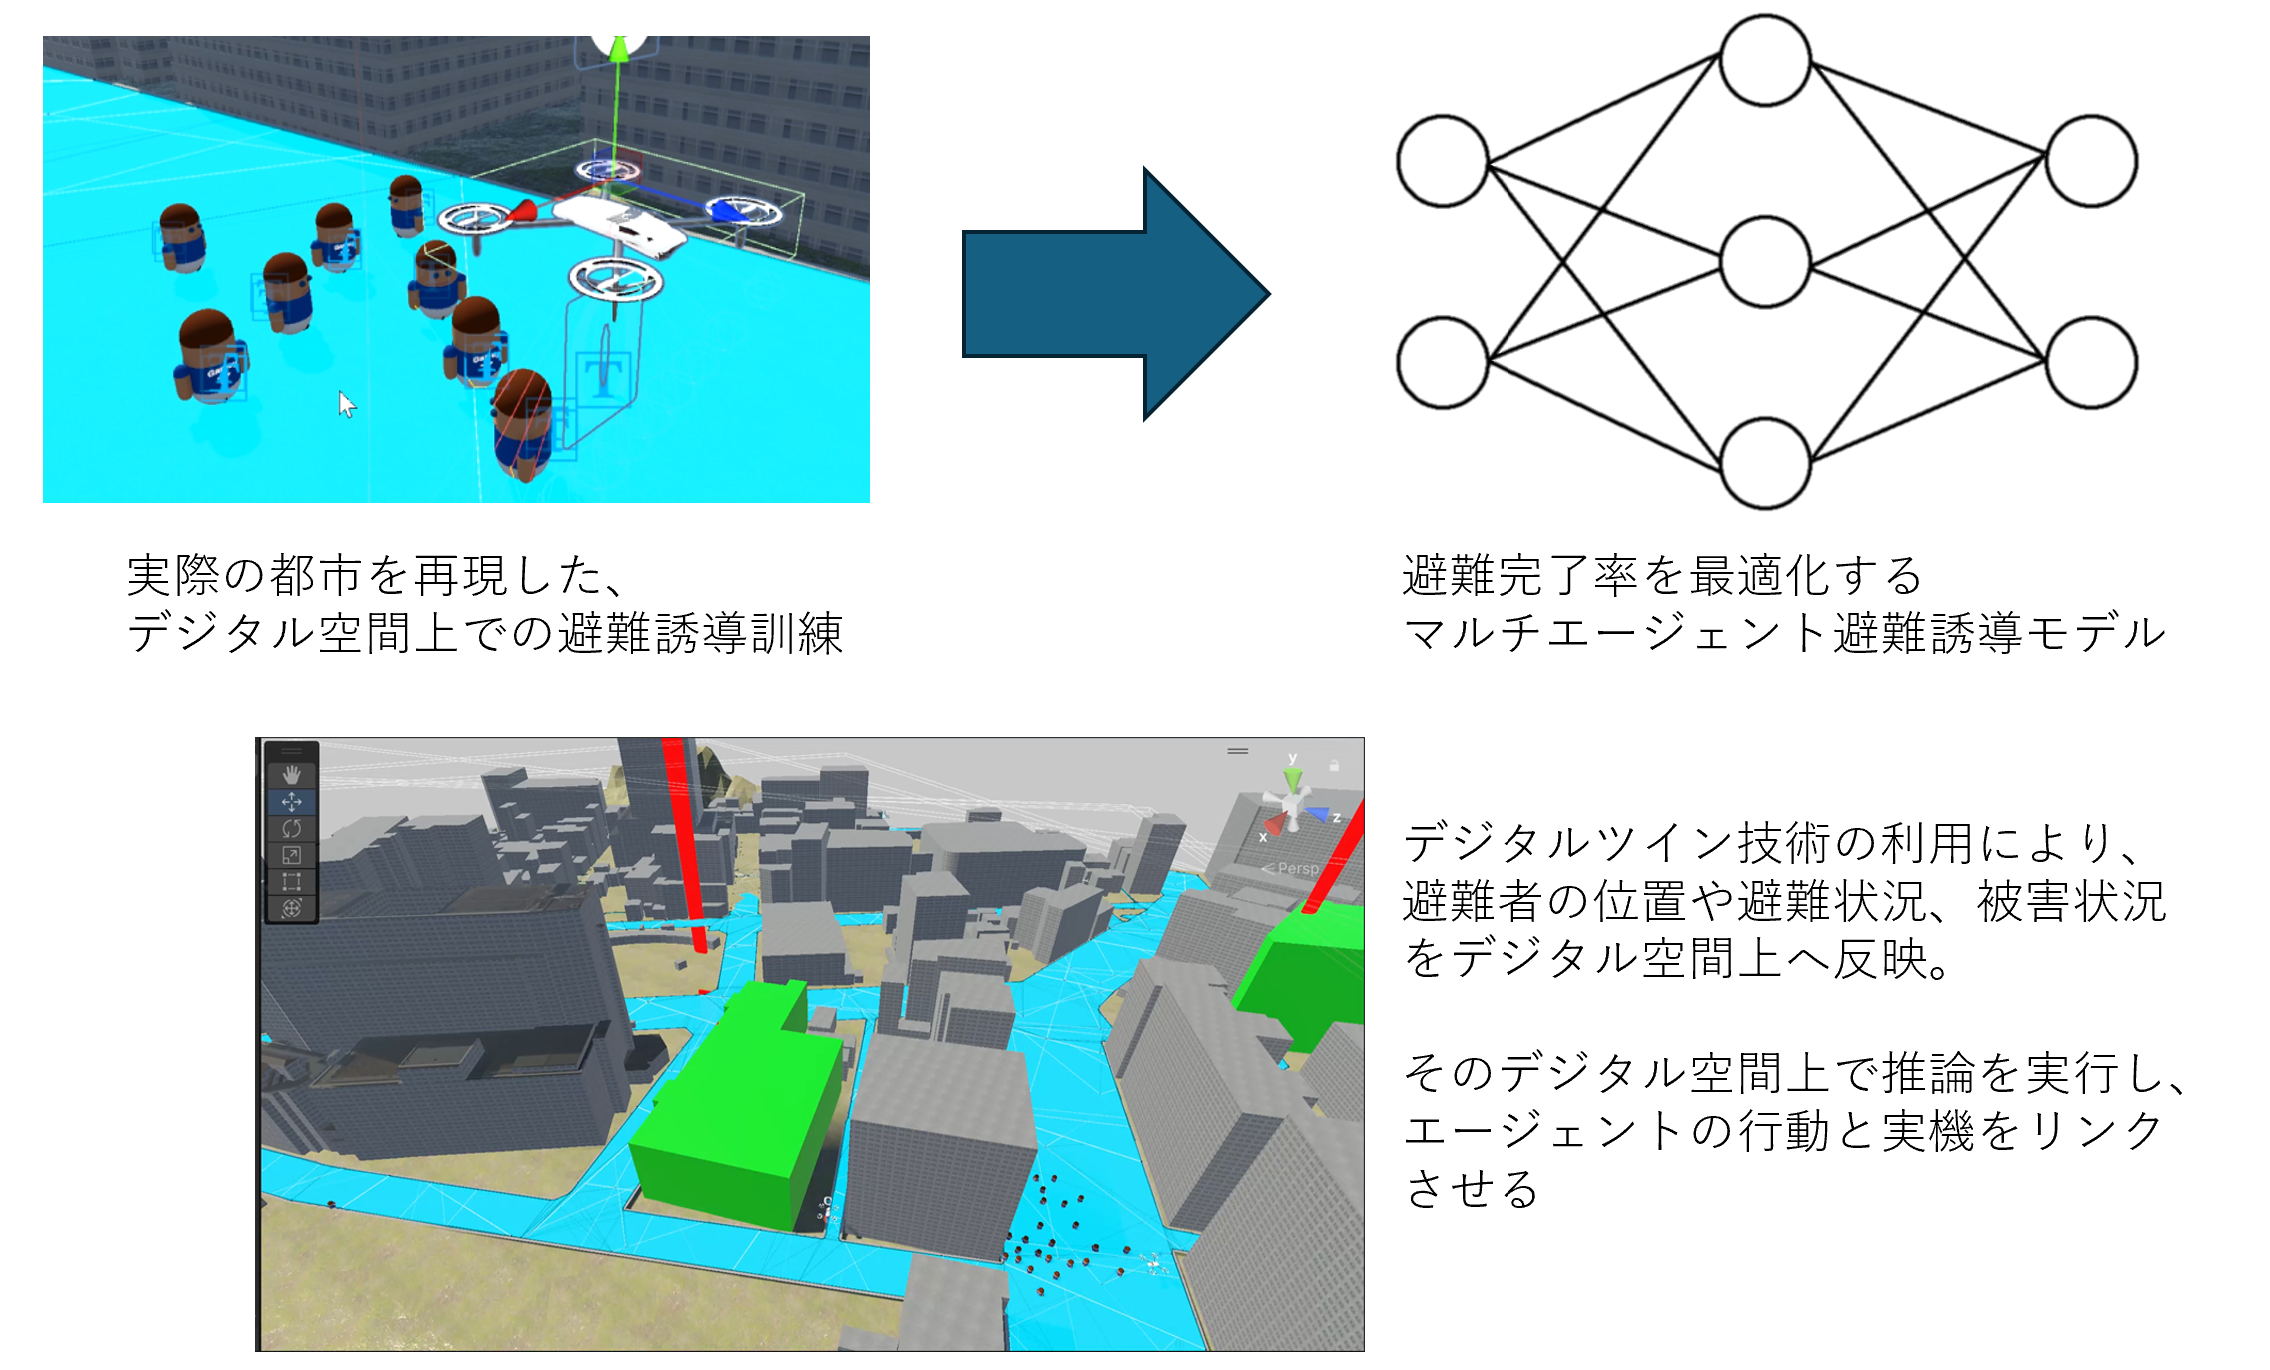
\includegraphics[width=1.0\textwidth]{Figures/2024-12-06 182816.png}
  \caption{提案手法 概略図} 
  \label{fig:01} 
\end{figure}

\section{既存研究との新規性}  
研究背景で述べたとおり,本研究は既存の研究といくつかの重要な相違点や新規性を有している.

まず,ドローンの防災活用はまだ研究が始まったばかりの新しい分野であり,本研究はその発展に寄与するものである.特に,複数のドローンを連携して運用するシステムに,AIや強化学習モデルを導入する点は,本研究の独自性を示す重要な要素である.

さらに,本研究では都市モデルを活用した訓練環境を構築し,デジタルツイン技術を通じて現実環境における運用を想定している.このように,現実世界での実用性を考慮した研究は,防災分野においても新しい試みである.

また,本研究は避難ビルの収容定員など,経路条件以外の要素を考慮した避難誘導モデルの作成にも取り組んでいる.
従来の研究の多くが,避難者自身の行動最適化を通じて避難完了率の向上を目指しているのに対し,本研究では避難完了率を最適化できる避難誘導方策そのものを追求している点で特徴的である.

以上のような取り組みにより,本研究は現実世界での応用可能性を持つ動的な津波避難誘導システムの実現を目指している.

\section{実験概要}
本研究では,津波避難誘導問題を解決するために,マルチエージェント強化学習を用いたドローン避難誘導システムを提案する.
本研究では、この問題を\textbf{1.避難者探索タスク}と\textbf{2.避難所誘導タスク}の2つの課題に分け、それぞれのタスクを解決するためのエージェントモデルをUnity上のシミュレーションにより構築する.
エージェントの訓練環境は実際の道路状況や避難所配置に限りなく近づけるため,都市モデルを活用したデジタルツイン環境を利用する.その後訓練済みエージェントモデルを利用した場合とルールベースで行動するエージェントを利用した場合それぞれのタスク遂行能力を評価するため,同一環境で比較シミュレーション実験を行う.
なお、2.避難所誘導タスクにおいては、ドローンエージェントの誘導がない場合,つまり避難者のみで避難行動を行う場合との比較も行う.
その実験結果から、最終的な避難完了率の推移や経過時間などの指標を用いて、提案手法の効果検証と実現可能性を評価する.

%TODO: 実験のイメージ図を追加
\section{シミュレーション前提条件}
\subsection{都市モデルの選定と避難所の配置条件}
環境としては,下記3つの都市の都市モデルをPLATEAU SDK for Unityを使い実際の都市環境に近いシミュレーション環境を再現する.
なお,都市の選定基準については,\ref{sec:sug}章にて述べた想定場面を考慮するため下記の選定基準をもって決定した.
\begin{enumerate}
  \item 南海トラフ等で津波被害が想定されている沿岸地域であること
  \item 自治体の津波避難のハザードマップが参照可能であること
  \item 地元住民以外にも多数の観光客が見込まれる,比較的規模の大きな地域であること
  \item 津波避難ビルあるいは津波避難タワーが整備されている地域であること
\end{enumerate}
以上の条件を元に,下記3つの都市をモデル都市として選択した.
\begin{enumerate}
  \item 神奈川県横須賀市 市役所本庁舎 周辺沿岸地域
  \item 静岡県沼津市 沼津港周辺の一部地域
  \item %% TODO;追加実験
\end{enumerate}
都市モデルと実際の避難ビル(避難タワー)との位置付けは,自治体公表のハザードマップより目算により算出し,都市モデル上で指定した.
各モデル都市におけるシミュレーション対象範囲は以下地図の赤枠で示した範囲とする.
\begin{figure}[H]
  \centering
  % 左側の画像
  \begin{minipage}{0.45\textwidth}
      \centering
      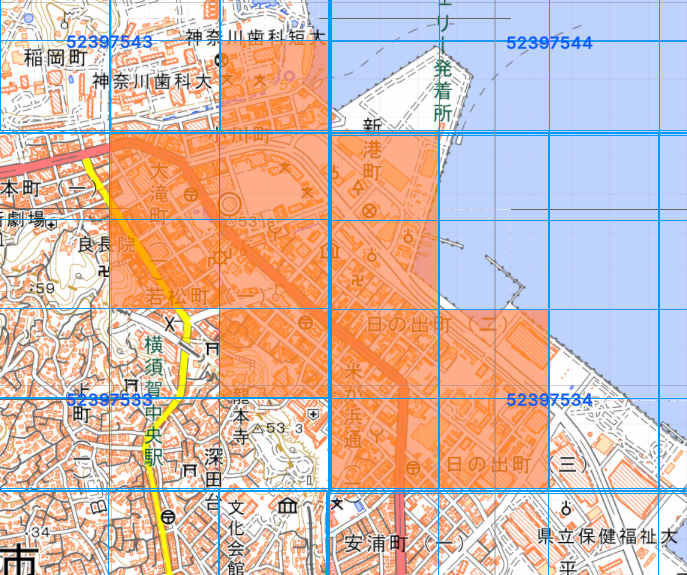
\includegraphics[width=\textwidth]{Figures/YokosukaMapRange.png} 
      \caption{横須賀市でのシミュレーション範囲}
      \label{fig:YokosukaMapRange}
  \end{minipage}
  \hfill % 隙間を調整
  % 右側の画像
  \begin{minipage}{0.45\textwidth}
      \centering
      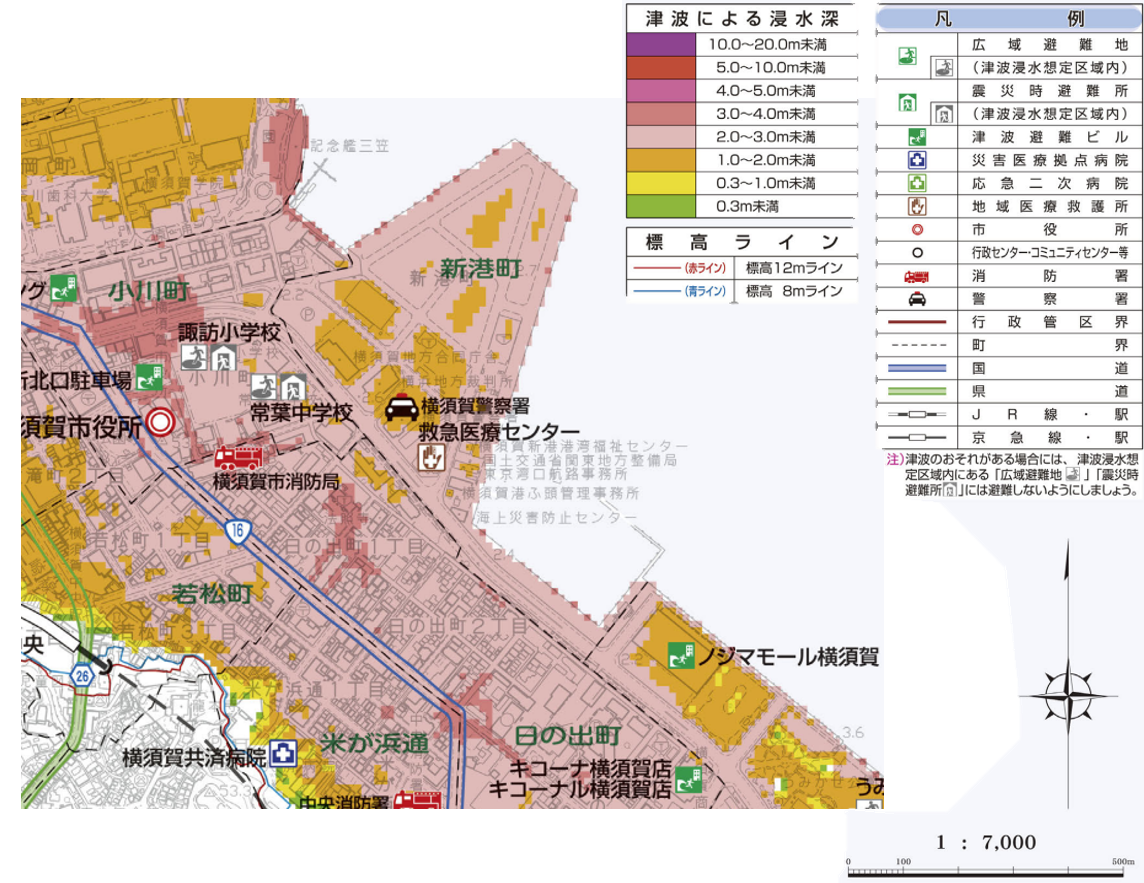
\includegraphics[width=\textwidth]{Figures/YokosukaHzaerd.png} 
      \caption{対象範囲の横須賀市のハザードマップ}
      \label{fig:right_image}
  \end{minipage}
\end{figure}

% TODO: 他の都市の図も追加
\subsection{避難者の前提条件}
避難者の初期出現位置は環境内の道路上にランダムに配置するものとする.避難者の移動方法は内閣府が公表している津波避難ガイドライン基づき徒歩移動ないしは自転車による移動を想定する.
そのため避難者の移動速度は,1m/sから3.4m/sの範囲内でランダムに設定する.
移動経路については、ナビゲーションメッシュにより指定位置までの道路上における最短経路を計算し,各避難者はその経路に従って移動するものとする.
\subsection{エージェントの前提条件}
エージェントの初期位置は,避難者の初期位置と同様に環境内の道路上にランダムに配置するものとする.なお,出現するエージェントの数は,環境内の避難所1つあたりにつき1機とする.
移動方法の詳細は後述する各実験の章にて述べる.
なお,強化学習アルゴリズムにはMA-POCAを利用する.

\section{避難者探索タスク実験の方法}
この実験ではエージェントは環境内の避難者を探索し,制限時間以内にできるだけ多くの避難者を見つけるタスクを行う.
\section{避難所誘導タスク実験の方法}
この実験ではエージェントは事前に割り当てられた避難者グループを指定された避難所まで誘導するタスクを行う.
シミュレーション開始時、エージェントは環境内のランダムな道路上に配置される.そのエージェントの周辺に10人から40人の避難者がランダムな人数配置される.
次にエージェントは観測として自身の環境内での位置情報や割り当てられている避難者の人数、各避難所までの移動距離や収容人数などの情報を取得する.その観測に基づいてエージェントは行動として,自身の移動速度を$1.0m/s$から$3.0m/s$の間で,誘導先である避難所を1つ決定し移動することができる.
避難者はエージェントに追従し,避難所に到達すると避難者は避難所に収容される.なお,避難所に収容される避難者の数は避難所の収容人数を超えることはないものとする.
もし,避難時点でその避難所の収容定員を超える場合,避難者はエージェントに追従し続け、次のエージェントの行動決定まで待機する.
制限時間を超えるか全ての避難者が避難所に収容された時にシミュレーションは終了する.
\subsection{エージェントの観測}
エージェントは環境内の以下の情報を観測することができる.
\begin{itemize}
  \item 自身の位置情報(X,Y,Z座標)
  \item 自身の移動速度(浮動小数値)
  \item 割り当てられている避難者の人数
  \item 避難者グループの平均移動速度
  \item 各避難所の位置情報(X,Y,Z座標)
  \item 各避難所までの移動距離
  \item 各避難所の現在の収容可能人数
  \item 他のエージェントの情報
  \begin{itemize}
    \item 他のエージェントの位置情報(X,Y,Z座標)
    \item 他のエージェントが移動する避難所の位置情報(X,Y,Z座標)
    \item 他のエージェントが誘導している避難者の人数
  \end{itemize}
\end{itemize}
  
 
\subsection{エージェントの行動}
エージェントは観測情報に基づいて以下の行動を取ることができる.
\begin{itemize}
  \item 移動先の避難所
  \item 自身の移動速度
\end{itemize}

\subsection{エージェントの報酬}
各エージェントは誘導した避難所に自身に割り当てられている避難者が到達するとその人数に応じて$+1$の正の個別報酬を得る.
また,グループ報酬として,シミュレーション終了時点での最終的な避難完了率を計算し,その値に応じて$0$~$1$の正のグループ報酬を得る.

\subsection{評価と比較}
この実験では,マルチエージェント強化学習を用いたエージェントモデルとルールベースで行動するエージェントモデル,避難者単独行動のパターンの3つの行動パターンを比較する.
ルールベースで行動するエージェントモデルは,自身から最も近い受け入れ可能な避難所までの最短経路を計算し,避難所に到達するまでの移動速度を一定に設定するものとする.
避難者単独のパターンでは、各避難者は自身から最寄りの避難所までの最短経路を計算し,その経路に従って移動するものとする.なおこの時避難者は、移動先の避難所の収容人数を知ることはできず,避難所に到達した段階で収容可能人数を超える場合,次の最寄りの避難所に向かうものとする.\par

以上の3つの行動パターンにおいて,避難完了率,避難所到達までの経過時間,などの指標を用いて,マルチエージェントモデルの有効性を評価する.